\documentclass[10pt,aspectratio=169]{beamer}

% --- Theme ---
\usetheme{metropolis}
\metroset{progressbar=none, numbering=fraction, block=fill}

% --- Packages ---
\usepackage[utf8]{inputenc}
\usepackage{graphicx}
\usepackage{booktabs}
\usepackage{tikz}
\usetikzlibrary{arrows.meta, positioning}
\usepackage{xcolor}
\usepackage{colortbl}
\usepackage{amsmath}
\usepackage{amssymb}
\usepackage{bookmark}
\usepackage{tcolorbox}

\graphicspath{{figures/}}

% --- Colors (matching deck2-deck7) ---
\definecolor{good}{RGB}{44,160,44}
\definecolor{bad}{RGB}{214,39,40}
\definecolor{warn}{RGB}{255,140,0}
\definecolor{accent}{RGB}{31,119,180}
\definecolor{idx}{RGB}{122,31,162}
\newcommand{\gd}[1]{\textcolor{good}{#1}}
\newcommand{\bd}[1]{\textcolor{bad}{#1}}
\newcommand{\wn}[1]{\textcolor{warn}{#1}}
\newcommand{\ix}[1]{\textcolor{idx}{#1}}
\newcommand{\code}[1]{{\small\texttt{#1}}}

% --- Title metadata ---
\title{Theme Detection --- updates VIII}
\subtitle{A first baseline, bag-of-words only: from detection to a backtested basket}
\date{August 2026}

\begin{document}

% =====================================================================
\begin{frame}[plain]
  \titlepage
  \vspace{-1.9cm}
  \begin{center}\scriptsize
  \begin{minipage}{0.88\textwidth}\centering
  The chain now runs end to end. Everything in this deck uses \textbf{words alone} ---
  no prices, no fundamentals, no tuning --- so it is the \textbf{floor} every smarter
  version must beat. Two worked examples (quantum, genAI) against the S\&P\,500.
  \end{minipage}
  \end{center}
\end{frame}

% =====================================================================
\begin{frame}[t]{The pipeline --- last stage is new (1/10)}
  \footnotesize
  \begin{center}
  \resizebox{\textwidth}{!}{%
  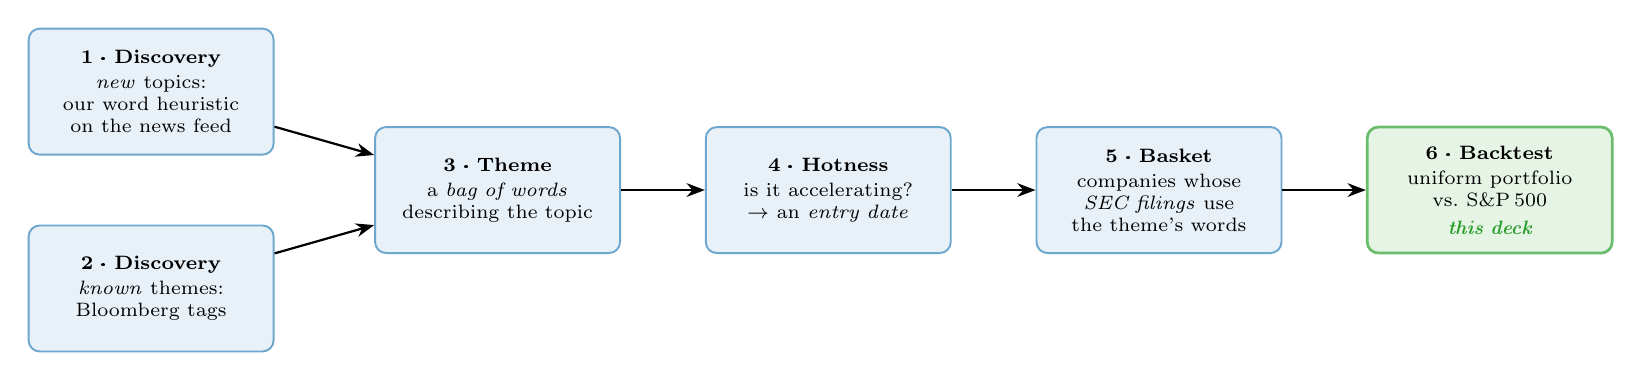
\begin{tikzpicture}[font=\scriptsize,>=Stealth,
     box/.style={draw,rounded corners,align=center,minimum height=1.6cm,text width=2.9cm,inner sep=3pt,
                 fill=accent!10,draw=accent!65,line width=0.7pt},
     hot/.style={draw,rounded corners,align=center,minimum height=1.6cm,text width=2.9cm,inner sep=3pt,
                 fill=good!12,draw=good!70,line width=1.0pt}]
    \node[box] (d1) at (0, 1.25)  {\textbf{1 · Discovery}\\[1pt] \emph{new} topics:\\ our word heuristic\\ on the news feed};
    \node[box] (d2) at (0,-1.25)  {\textbf{2 · Discovery}\\[1pt] \emph{known} themes:\\ Bloomberg tags};
    \node[box] (th) at (4.4, 0)  {\textbf{3 · Theme}\\[1pt] a \emph{bag of words}\\ describing the topic};
    \node[box] (mon) at (8.6, 0) {\textbf{4 · Hotness}\\[1pt] is it accelerating?\\ $\to$ an \emph{entry date}};
    \node[box] (bk) at (12.8, 0) {\textbf{5 · Basket}\\[1pt] companies whose\\ \emph{SEC filings} use\\ the theme's words};
    \node[hot] (bt) at (17.0, 0) {\textbf{6 · Backtest}\\[1pt] uniform portfolio\\ vs.\ S\&P\,500\\[2pt] {\itshape\color{good}\textbf{this deck}}};
    \draw[->,thick] (d1) -- (th);
    \draw[->,thick] (d2) -- (th);
    \draw[->,thick] (th)  -- (mon);
    \draw[->,thick] (mon) -- (bk);
    \draw[->,thick] (bk) -- (bt);
  \end{tikzpicture}}
  \end{center}

  \vspace{0.25cm}
  \textbf{What this baseline is.} Words all the way through: words discover the theme,
  words date its acceleration, words (counted in SEC filings) pick the companies. The
  portfolio is uniform and the backtest has no free parameters. Deliberately the simplest
  thing that could work --- so the two examples measure the \emph{method}, not our tuning.
\end{frame}

% =====================================================================
\begin{frame}[t]{Detection: two routes to a theme, one hotness score (2/10)}
  \footnotesize
  \begin{columns}[T,onlytextwidth]
    \column{0.55\textwidth}
      \textbf{New themes --- the word-novelty heuristic.} A theme being born mints new
      vocabulary. We keep the words never seen in a two-year baseline and promote those that
      cluster, persist and bridge across headlines:
      \[
        \text{candidates} \to \text{caught} \to \text{promoted}
      \]
      \gd{genAI: \emph{chatgpt} caught in the week of Jan\,3\,2023, promoted Jan\,17 ---
      seven weeks after launch, four months before the first genAI ETF.}

      \vspace{0.15cm}
      \textbf{Known themes --- Bloomberg tags.} If a topic code already exists, the tag
      \emph{is} the theme definition and we skip discovery entirely.
    \column{0.42\textwidth}
      \begin{block}{Hotness}
        \scriptsize
        Either way, the theme's temperature is the rolling z-score of its weekly headline
        count,
        \[
          z_t = \frac{c_t - \mu_{t-1}}{\sigma_{t-1}},
        \]
        which ranks competing themes and gives the \textbf{entry date} for the backtest.
      \end{block}
      \begin{block}{Why both routes}
        \scriptsize
        The heuristic sees themes \emph{before} any tag exists; tags cover mature themes at
        zero cost.
      \end{block}
  \end{columns}
\end{frame}

% =====================================================================
\begin{frame}[t]{Portfolio: uniform weights, on purpose (3/10)}
  \footnotesize
  \textbf{Basket.} A company enters if its annual/quarterly SEC reports mention the theme's
  words (point-in-time: only filings available at the entry date). Rank by mention counts,
  keep the top names. The rule can also refuse: \gd{at the 2018 quantum-ETF date it selects
  \emph{zero} companies --- no investable theme, no trade.}

  \vspace{0.25cm}
  \textbf{Weights.} At every rebalance date each of the $N$ held names gets
  \[
    w_j = \tfrac{1}{N} \qquad \text{(equal euros per name).}
  \]
  Uniform needs no estimates and no optimizer --- the right property for a floor. Note that
  resetting to $1/N$ each quarter means \textbf{selling the quarter's winners to buy its
  losers}: a real economic choice, whose cost we measure on slide 7.

  \vspace{0.25cm}
  \textbf{Prices.} Split- and dividend-adjusted daily closes, so price ratios always compare
  comparable per-share values (verified on NVDA's 2024 10-for-1 split: no discontinuity).
\end{frame}

% =====================================================================
\begin{frame}[t]{Backtest: four formulas, no knobs (4/10)}
  \footnotesize
  Buy at the theme's entry date, hold $m$ months, rebalance, repeat. Periods are
  \textbf{contiguous}: each exit day \emph{is} the next entry day --- no return falls between.

  \begin{columns}[T,onlytextwidth]
    \column{0.55\textwidth}
    Time runs on a \textbf{grid of rebalance days}, not continuously: $t_i$ = first trading
    day $\ge$ entry $+\ i\cdot m$ months, for $i = 0,\dots,n$, with $t_n$ = end date.
    Period $i$ goes from $t_i$ to $t_{i+1}$ and its return uses \emph{only those two
    endpoints}, equal-weighted over the held names $H_i$ (basket members with a price at $t_i$):
    \[
      r_i = \frac{1}{|H_i|} \sum_{j \in H_i} \Bigl( \frac{P_j(t_{i+1})}{P_j(t_i)} - 1 \Bigr),
      \qquad i = 0,\dots,n-1
    \]
    \[
      R = \sum_i r_i, \qquad \sigma = \operatorname{std}(r_i), \qquad
      \text{ratio} = \frac{R}{\sigma},
    \]
    \[
      \text{Sharpe}_{\text{ann}} = \frac{\bar r}{\sigma}\,\sqrt{12/m},
    \]
    where $m$ is the rebalance interval in months, so $12/m$ = periods per year
    (here $m=3$: $\sqrt{12/3}=2$).
    \column{0.42\textwidth}
      \begin{block}{Which ratio when}
        \scriptsize
        $R/\sigma$ grows with the number of periods: fair only \emph{within} one window.
        The annualized Sharpe is horizon-free --- it is how we compare experiments with
        different entry dates.
      \end{block}
      \begin{block}{Benchmark}
        \scriptsize
        The S\&P\,500 (dividend-adjusted, via SPY) runs through the \emph{same} formula on
        the \emph{same} days --- apples to apples by construction.
      \end{block}
  \end{columns}
\end{frame}

% =====================================================================
\begin{frame}[t]{Example 1 --- quantum: detected early, paid late (5/10)}
  \footnotesize
  \begin{columns}[T,onlytextwidth]
    \column{0.52\textwidth}
      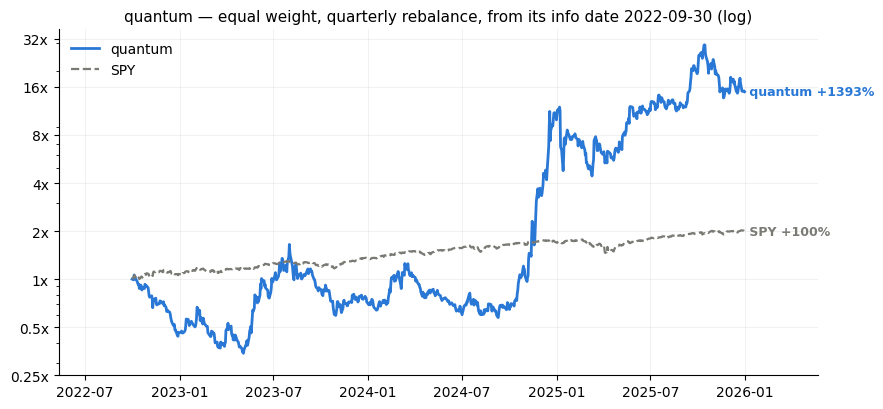
\includegraphics[width=\textwidth]{quantum_curve.png}
    \column{0.45\textwidth}
      Entry \textbf{2022-09-30}; the rule's four pure-plays (IONQ, QUBT, RGTI, QBTS);
      14 quarters.

      \vspace{0.1cm}
      {\scriptsize
      \begin{tabular}{@{}lrrrr@{}}
        \toprule
                 & sum $R$ & $\sigma$ & $R/\sigma$ & Sharpe \\
        \midrule
        quantum  & \gd{+1670\%} & \bd{406\%} & 4.1 & \bd{0.59} \\
        S\&P\,500 & +72\%  & 5.2\%  & 14.0 & \gd{2.00} \\
        quantum ETF & +126\% & 11.2\% & --- & 1.62 \\
        \bottomrule
      \end{tabular}}

      \vspace{0.15cm}
      First quarter after entry: \bd{$-54\%$}; a year below half the starting capital.
      \textbf{91\% of the sum is one quarter} (Q4-2024). The four names move together
      (correlation \bd{0.93}) --- effectively \emph{one} bet, so the basket carries full
      single-stock volatility. The diversified theme ETF shows what breadth alone buys: 1.62.
  \end{columns}

  \vspace{0.1cm}
  {\tiny \textbf{3M returns (\%)} --- quantum:
  $-54,\,-13,\,+140,\,-11,\,-19,\,+49,\,-42,\,+13,\,\bd{+1516},\,-45,\,+94,\,+65,\,-22,\,-1$
  \;·\; S\&P\,500: $+8,\,+6,\,+10,\,-3,\,+11,\,+11,\,+5,\,+6,\,+3,\,-5,\,+11,\,+8,\,+3,\,-1$}
\end{frame}

% =====================================================================
\begin{frame}[t]{Example 2 --- genAI: detected on time, mapped to the wrong companies (6/10)}
  \footnotesize
  \begin{columns}[T,onlytextwidth]
    \column{0.52\textwidth}
      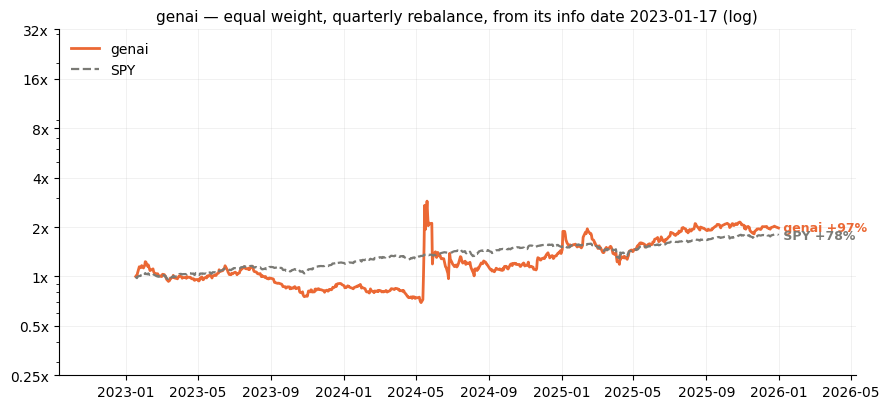
\includegraphics[width=\textwidth]{genai_curve.png}
    \column{0.45\textwidth}
      Entry \textbf{2023-01-17} (the promotion week); point-in-time top-10 from SEC
      filings (NVDA, TRIP, GOOG, EA, MYPS, APPS, EXPE, EBAY, CRNC, FFAI); 12 quarters.

      \vspace{0.1cm}
      {\scriptsize
      \begin{tabular}{@{}lrrrr@{}}
        \toprule
               & sum $R$ & $\sigma$ & $R/\sigma$ & Sharpe \\
        \midrule
        genAI  & \gd{+101\%} & \bd{26\%} & 3.9 & \bd{0.64} \\
        S\&P\,500 & +62\%  & 7.6\% & 8.2 & \gd{1.36} \\
        \bottomrule
      \end{tabular}}

      \vspace{0.15cm}
      The theme was \textbf{seven weeks old}: no filing mentioned its vocabulary yet, so
      word counts picked pre-ChatGPT ``AI-talkers'' --- travel portals, e-commerce, and the
      meme stock behind the orange spike. NVDA alone is 101pp of the basket's 133pp; the
      other nine add volatility, not theme.
  \end{columns}

  \vspace{0.1cm}
  {\tiny \textbf{3M returns (\%)} --- genAI:
  $-1,\,+15,\,-25,\,-2,\,-10,\,\wn{+67},\,-6,\,+30,\,-14,\,+43,\,+8,\,-3$
  \;·\; S\&P\,500: $+5,\,+9,\,-3,\,+9,\,+6,\,+12,\,+5,\,+3,\,-12,\,+20,\,+6,\,+3$}
\end{frame}

% =====================================================================
\begin{frame}[t]{Results: high return, higher volatility (7/10)}
  \footnotesize
  Both baskets beat the S\&P\,500 by a wide margin on raw return --- and both lose to it
  once risk is counted, in a window where the index's own Sharpe sits at the \textbf{90th
  percentile} of its history (median 3-year Sharpe since 1994: 1.0).

  \vspace{0.15cm}
  \begin{columns}[T,onlytextwidth]
    \column{0.48\textwidth}
      \begin{block}{Where the risk comes from}
        \scriptsize
        \textbf{Quantum}: concentration --- four names, correlation 0.93, one bet at
        400\%/quarter volatility.\\[2pt]
        \textbf{genAI}: two lottery tickets dominate the volatility budget, and quarterly
        rebalancing keeps re-buying them after each collapse --- that alone costs
        \bd{0.33 of Sharpe} vs.\ buy-and-hold of the same list (0.97).
      \end{block}
    \column{0.48\textwidth}
      \begin{block}{How fragile}
        \scriptsize
        Drop each basket's best quarter: Sharpe $0.59 \to 0.40$ (quantum),
        $0.64 \to 0.32$ (genAI). The index barely moves. One quarter carries everything.
      \end{block}
      \begin{block}{The words were right --- in the news}
        \scriptsize
        The co-mention basket (slide 10) beats the index (1.94 vs.\ 1.37):
        the \emph{mapping}, not the words, was genAI's problem.
      \end{block}
  \end{columns}
\end{frame}

% =====================================================================
\begin{frame}[t]{Limits (8/10)}
  \footnotesize
  \begin{enumerate}\itemsep 7pt
    \item \bd{\textbf{Only positive themes so far.}} Quantum and genAI are themes we know
      exploded --- selection bias by construction. How often the pipeline buys a theme that
      \emph{dies} is unmeasured, and it is the question that matters.
    \item \bd{\textbf{Words are not sufficient on SEC filings for newborn themes.}}
      Filings lag the news by months: at genAI's entry date its vocabulary existed in no
      filing, so counts selected noise. The same words applied to the news worked
      (Sharpe 1.94--1.99). Filings remain valid for mature themes --- quantum's four
      pure-plays were found without naming them.
    \item \bd{\textbf{No exit rule yet.}} Detection gives an \emph{entry} date; nothing tells
      us when the theme is over, so the backtest simply holds to the end of the window.
      Quantum shows what is at stake: sell after the crash and the theme is a disaster, hold
      through it and it is the best trade in the deck. The natural candidate --- hotness
      decay as an exit signal --- is untested.
    \item \textbf{Smaller prints.} No transaction costs or market impact (microcaps!);
      early quantum quarters trade pre-merger SPAC prices; every Sharpe here rests on one
      quarter and is a fragile point estimate.
  \end{enumerate}
\end{frame}

% =====================================================================
\begin{frame}[t]{Next: the backtest becomes the judge (9/10)}
  \footnotesize
  Stop asking ``does one basket beat the index'' --- run the whole chain over \emph{many}
  themes and dates, including the duds, and let the outcome label each theme:
  \[
    \text{theme} \;\longmapsto\; (\text{Sharpe},\, R,\, \sigma,\, \text{drawdown})
    \;\longmapsto\; \{\gd{\text{good}},\, \bd{\text{bad}}\}
  \]

  \vspace{0.1cm}
  \begin{columns}[T,onlytextwidth]
    \column{0.48\textwidth}
      \begin{block}{What the labels buy us}
        \scriptsize
        The real question becomes answerable: \emph{which detection-time features predict a
        good theme?} Hotness, novelty type, basket purity, concentration, breadth of the
        co-mention graph --- a classifier trained on our own backtests.
      \end{block}
    \column{0.48\textwidth}
      \begin{block}{Supporting fixes}
        \scriptsize
        Map newborn themes through the news co-mention graph (filings only for mature ones);
        add simple risk caps to the uniform baseline; keep negative-control themes in the
        set to keep the classifier honest.
      \end{block}
  \end{columns}
\end{frame}

% =====================================================================
\begin{frame}[t]{genAI, take two: the detection's co-mentions as the basket (10/10)}
  \footnotesize
  \begin{columns}[T,onlytextwidth]
    \column{0.50\textwidth}
      Each week the funnel also lists the words \emph{co-mentioned} with the anchor ---
      from the genAI run, in order of appearance:

      \vspace{0.1cm}
      {\scriptsize
      \begin{tabular}{@{}ll@{}}
        \toprule
        week (2023) & new co-mentions of \emph{chatgpt} \\
        \midrule
        Jan 3--9            & microsoft \\
        Jan 17--23 \emph{(promotion)} & openai \\
        Jan 24--30          & \textbf{nvidia}, altman \\
        Jan 31--Feb 6       & \textbf{google} (Bard) \\
        Feb 7--13           & baidu, alibaba, netease (Ernie) \\
        Feb 21--27          & amazon (Hugging Face) \\
        \bottomrule
      \end{tabular}}

      \vspace{0.1cm}
      Listed ones only, mapped to tickers: \textbf{core} = MSFT, NVDA, GOOGL (enter
      Feb\,1) · \textbf{ecosystem} = +BIDU, BABA, NTES, AMZN (Mar\,1). \textbf{No SEC
      filings involved} --- vs.\ example 2 only the word$\to$company \emph{mapping} changed.
    \column{0.46\textwidth}
      {\scriptsize
      \begin{tabular}{@{}lrrr@{}}
        \toprule
                      & sum $R$ & $\sigma$ & Sharpe \\
        \midrule
        core (3)      & +160\% & 13.8\% & \gd{\textbf{1.94}} \\
        S\&P\,500 (same window) & +59\%  & 7.1\%  & 1.37 \\
        \addlinespace[2pt]
        ecosystem (7) & +106\% & 8.8\%  & \gd{1.99} \\
        S\&P\,500 (same window) & +61\%  & 4.3\%  & 2.37 \\
        \bottomrule
      \end{tabular}}

      \vspace{0.1cm}
      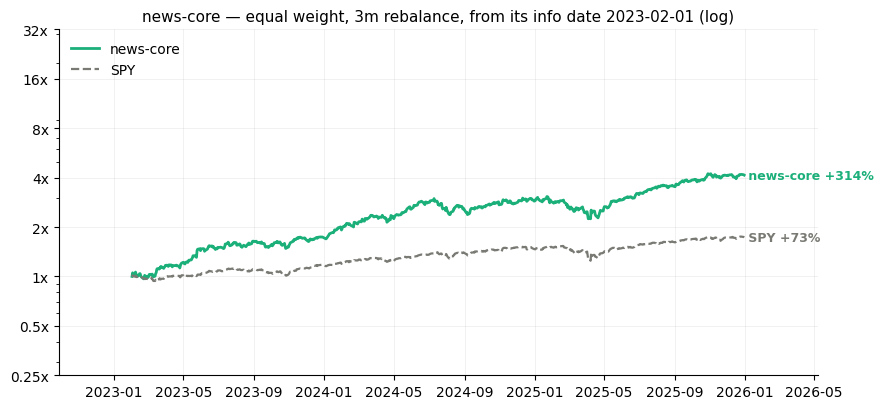
\includegraphics[width=\textwidth]{newscore_curve.png}
  \end{columns}

  \vspace{0.1cm}
  {\tiny \textbf{3M returns (\%)} --- news-core:
  $+22,\,+31,\,-3,\,+26,\,+15,\,+14,\,+8,\,+1,\,-7,\,+32,\,+23,\,-2$
  \;·\; S\&P\,500: $+2,\,+10,\,-7,\,+16,\,+3,\,+9,\,+5,\,+5,\,-6,\,+12,\,+10,\,+0$}
\end{frame}

\end{document}
